\begin{figure*}[t]
\centering
\vspace*{-1.5em}
%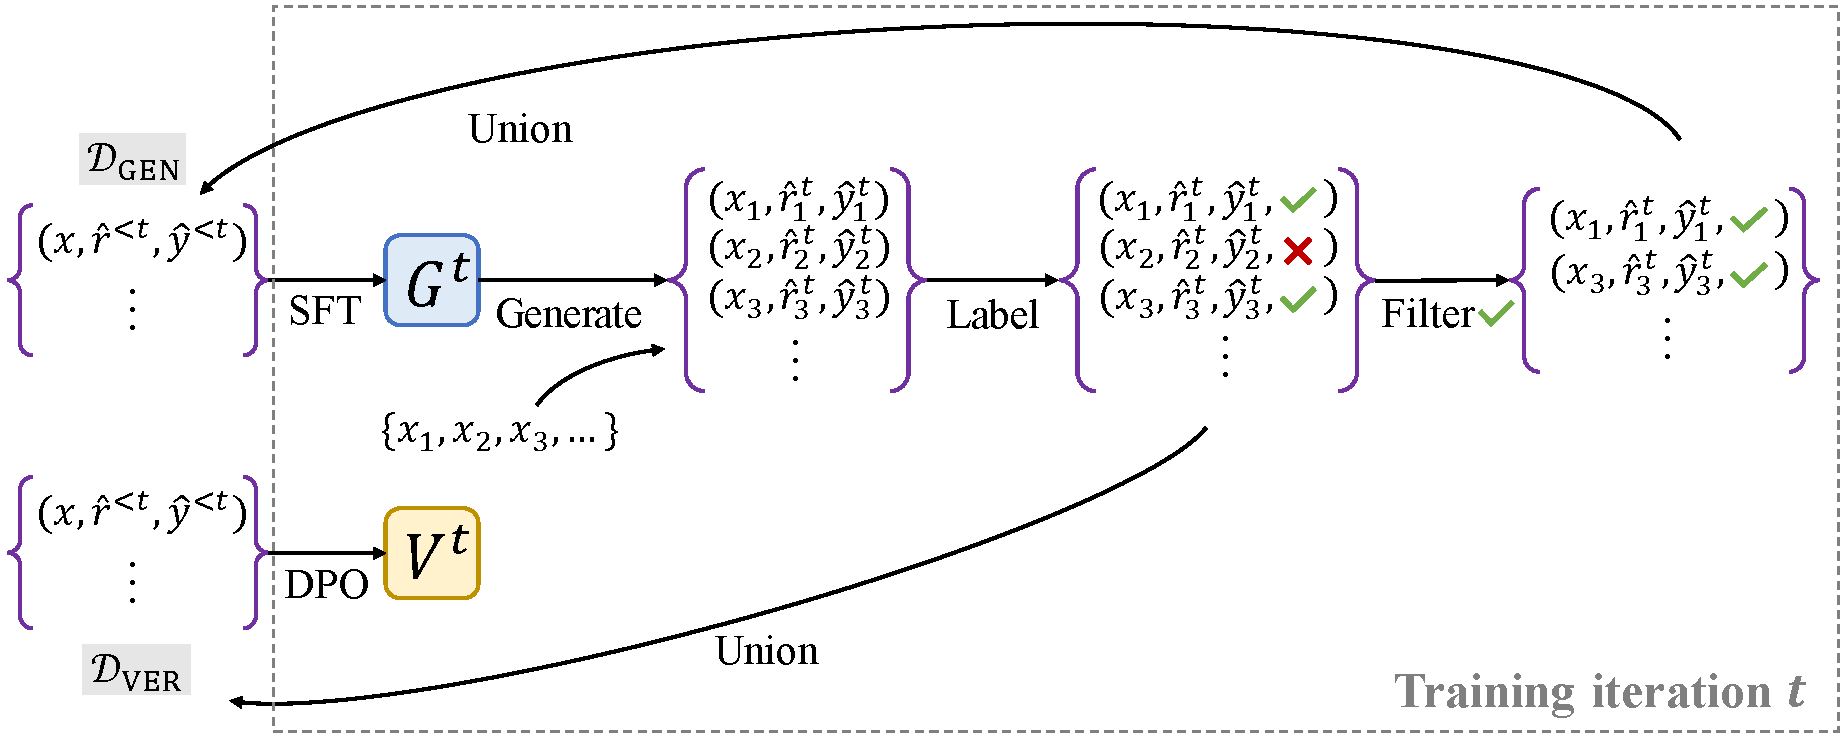
\includegraphics[width=0.66\linewidth]{icml2023/figs/v_star_intro_train.pdf}
%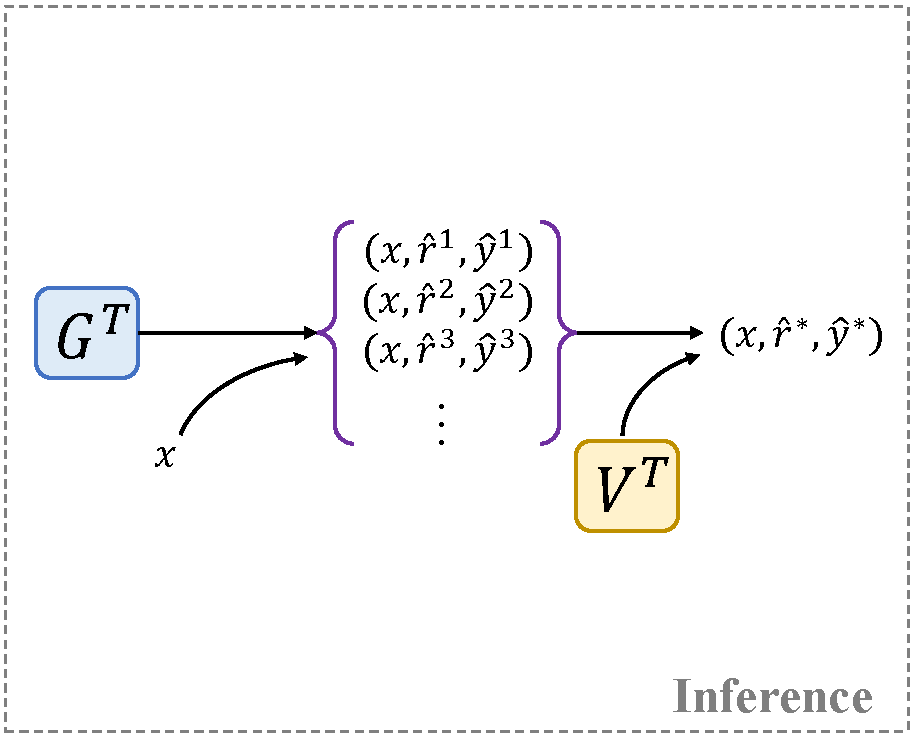
\includegraphics[width=0.328\linewidth]{icml2023/figs/v_star_intro_inference.pdf}
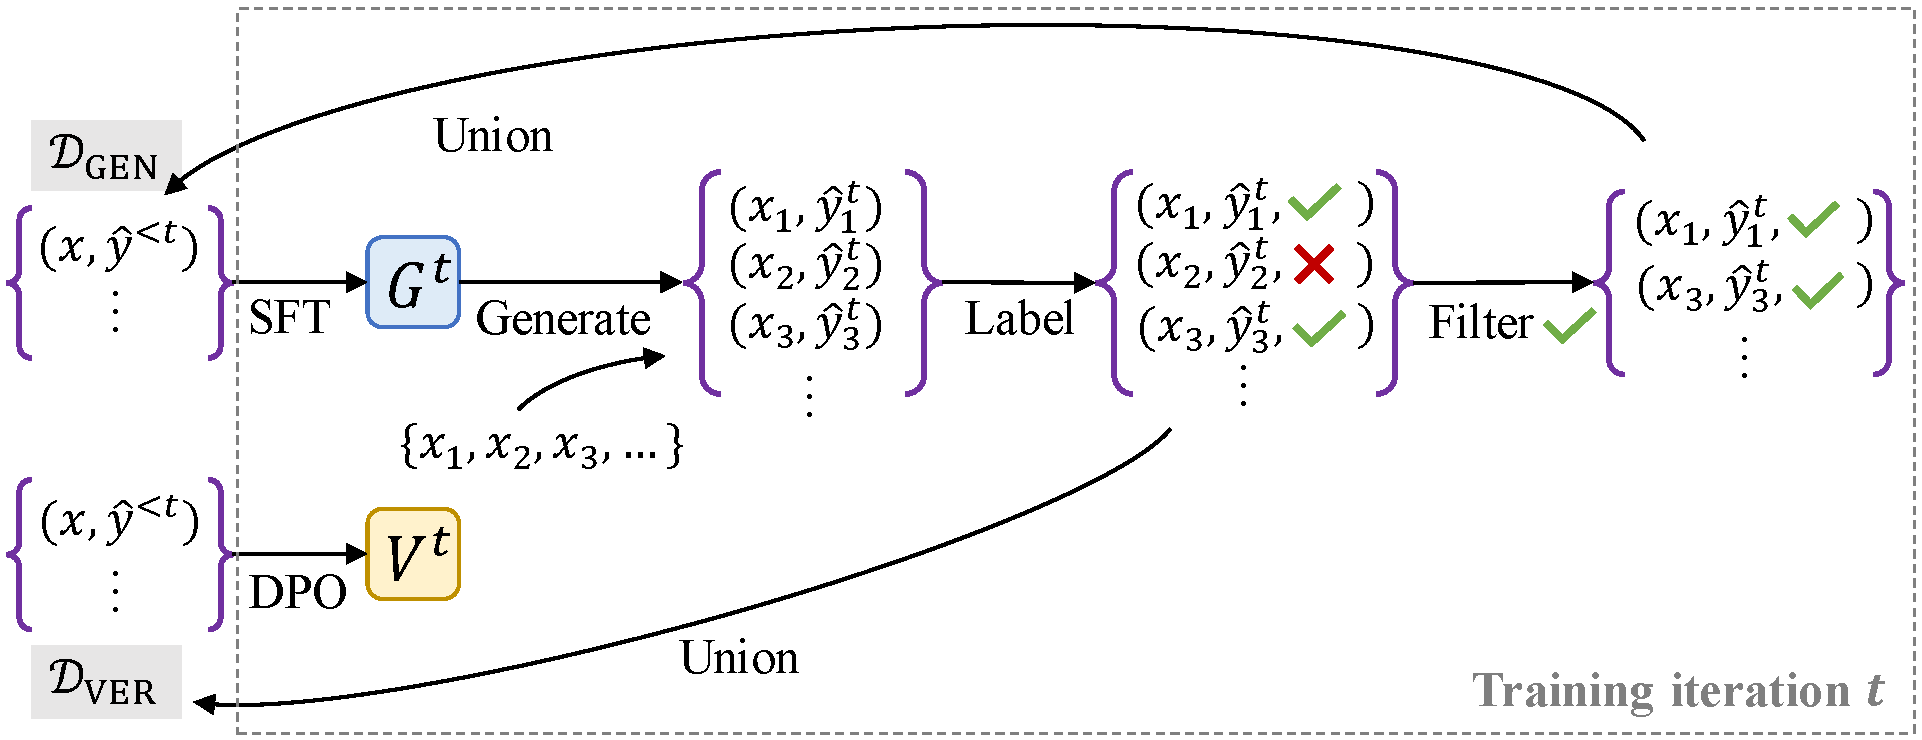
\includegraphics[width=0.674\linewidth]{icml2023/figs/v_star_intro_train_wo_r.pdf}
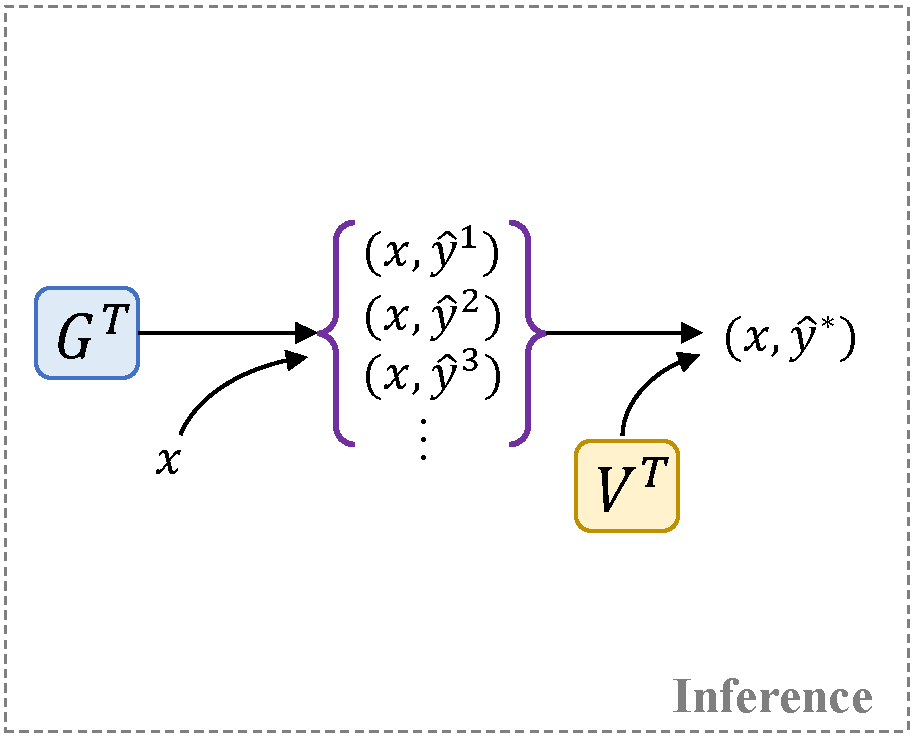
\includegraphics[width=0.32\linewidth]{icml2023/figs/v_star_intro_inference_wo_r.pdf}
\caption{\textbf{Generator and verifier training in \vstar{}}. \textbf{Left:} In each training iteration, the generator $G^t$ is fine-tuned (from a pretrained LLM) on the current buffer of problem instances and correct solutions ${\cal D}_{\text{GEN}}$. Generated solutions that yielded a correct answer are added to ${\cal D}_{\text{GEN}}$ to be used in future iterations, and all the generated solutions (correct and incorrect) are added to ${\cal D}_{\text
{VER}}$. The verifier $V^t$ is trained using DPO with a preference dataset constructed from pairs of correct and incorrect solutions from ${\cal D}_{\text{VER}}$. \textbf{Right:} At test time, the verifier is used to rank solutions produced by the generator. Such iterative training and inference-time ranking yields large improvements  over generator-only self-improvement.}
\label{fig:method}
\end{figure*}